\documentclass[10pt,a4paper]{report}

%Packages
\usepackage[utf8]{inputenc}
\usepackage[margin=1in]{geometry}
\usepackage{amsmath,amsfonts,amssymb,amsthm}
\usepackage[english]{babel}
\usepackage{csquotes}
\usepackage{chngcntr}
\usepackage[titletoc]{appendix}
\usepackage{listings}
\usepackage{xcolor}

%Citations
\usepackage{biblatex}
\addbibresource{references.bib}

%Argmin and argmax
\DeclareMathOperator*{\argmax}{arg\,max}
\DeclareMathOperator*{\argmin}{arg\,min}

%Images and Graph Plots
\usepackage{graphicx}
\graphicspath{{figures/}}
\usepackage{tikz, pgf, pgfplots}
\pgfplotsset{width=10cm,compat=newest}
\usepgfplotslibrary{external}
\tikzexternalize[prefix=tikz/]

%Code Segments
\definecolor{codegreen}{rgb}{0,0.6,0}
\definecolor{codegray}{rgb}{0.5,0.5,0.5}
\definecolor{codepurple}{rgb}{0.58,0,0.82}
\definecolor{backcolour}{rgb}{0.95,0.95,0.92}

\lstdefinestyle{code}{
	backgroundcolor=\color{backcolour},
	commentstyle=\color{codegreen},
	keywordstyle=\color{magenta},
	numberstyle=\tiny\color{codegray},
	stringstyle=\color{codepurple},
	basicstyle=\ttfamily\footnotesize,
	breakatwhitespace=false,
	breaklines=true,
	captionpos=b,
	keepspaces=true,
	numbers=left,
	numbersep=5pt,
	showspaces=false,
	showstringspaces=false,
	showtabs=false,
	tabsize=2
}
\lstset{style=code}

%Hyperlinks
\usepackage[hidelinks, pdfpagelabels]{hyperref}
\hypersetup{pageanchor=true}

\setlength{\parindent}{0mm}
\setlength{\parskip}{2mm}

%Document Information
\title{What are the limitations of derivative-based \\
	   models for optimization in machine learning?}
\author{Faris Chaudhry}
\date{\today}

%Environments
\newtheorem{theorem}{Theorem}[chapter]
\newtheorem{lemma}[theorem]{Lemma}
\newtheorem*{definition}{Definition}
\counterwithout{equation}{chapter}

%Page Numbering
\newcommand\frontmatter{
	\cleardoublepage
	\pagenumbering{roman}}
\newcommand\mainmatter{
	\cleardoublepage
	\pagenumbering{arabic}}

\begin{document}
	\frontmatter
	\maketitle

	\begin{abstract}
		Most machine learning problems can be transposed into optimization problems
		where the goal is finding the global minima or maxima to minimize loss or maximize potential.
		Each of the main learning methodologies (namely supervised, unsupervised and reinforcement)
		along with the models to represent and solve optimization problems have limitations -
		computationally and theoretically - that have to be identified and mitigated against
		to create an effective model. The focus here is continuously differentiable objective functions
		and thus derivative-based solutions are used.
	\end{abstract}

	\tableofcontents
	\mainmatter

    \chapter{Introduction to Machine Learning and Optimization}

		\section{What is Machine Learning?}
			Machine learning (ML) is a subfield of artificial intelligence (AI) and,
			broadly speaking, is the use of computational methods and models to improve
			performance and predictions through experience \autocite[p. 1]{FoundationsOfMachineLearning}.
			Unlike humans, this learning is based entirely on data and statistics with
			experience being gained through interaction with a data set
			or an environment of some kind. \par
			\begin{figure}[h]
				\centering
				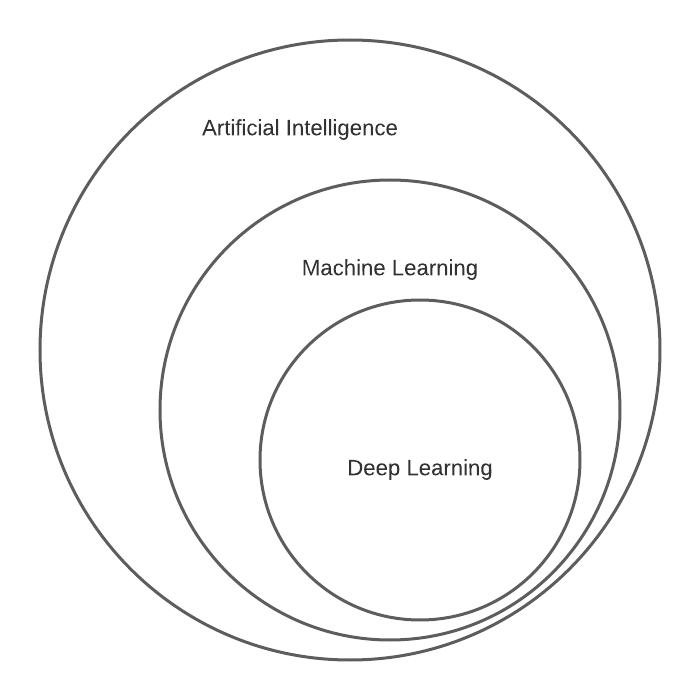
\includegraphics[scale=0.8]{ai-fields-euler-diagram.png}
				\caption{subfields of AI}
				\label{fig:ai-subfields}
			\end{figure}
			There are 3 primary categories of learning philosophies (supervised, unsupervised and reinforcement) for ML models,
			with other hybrid methods being combinations of these. Each type of learning lends itself to certain types of problems.
			Supervised learning is used for classifying images and extrapolating data. Unsupervised learning
			takes raw data and finds patterns such as the overall distribution or groups with similar attributes. Reinforcement is used in complex
			systems which many changing variables that would be computationally difficult to solve otherwise, like chess.

		\section{Prerequisite Conditions for Derivative-Based Optimization}
			Optimization revolves around minimizing the loss or maximizing the value of a function. In the
			context of ML, optimization is vital to ensure modelling produces the greatest accuracy.
			The goal is to optimize an objective function, which is the
			representation of the variables being simulated. The solution to the objective function will be
			either a minimum (minima) or maximum (maxima) point (collectively called the set of extrema) as
			this is when the value of a function is highest or lowest. \par
			The derivative is the linear approximation (tangent) to a function at a point. Suppose there was a
			function $f(x)$ then, intuitively, the derivative with respect to $x$ would be how much the value of $f(x)$
			changed with a small nudge in the $x$-direction. It is important to note that, by Fermat's theorem on stationary points
			\autocite{StationaryPoints}, all critical points (extrema and saddle points) have first derivative equal to 0. Visually, this
			is because the tangent to any turning point will have a gradient of 0. See the function $y = x^2$ (fig. \ref{fig:extrema}) which has a minima at $(0,0)$. \par
			\begin{figure}[h]
				\centering
				\begin{tikzpicture}
					\begin{axis}[
						width=5cm,
						height=5cm,
						xtick=\empty,
						ytick=\empty,
						xlabel=$x$,
						ylabel=$y$,
						axis lines=center,
						domain=-2.5:2.5,
						samples=100]
						\addplot [red] {x^2};
					\end{axis}
				\end{tikzpicture}
				\caption{graph of $x^2$}
				\label{fig:extrema}
			\end{figure}
			So the objective becomes to find the location and nature - whether it's an minima, maxima or saddle point - of each critical point.

			\subsection{Continuity and Differentiability}
				The most essential requirement to using derivative-based methods will be that the objective
				function is continuous and twice-differentiable (the derivative of the function must also be differentiable)
				over the interval that contains the solution. \par
				This is because to find the location and nature of critical points, the first and second derivative
				of a function are required \autocite{SecondDerivativeTest}. \par


				For a function $f(x)$ to be continuous over the interval $I = [a,b]$
				\begin{equation}
					\forall k \in I, \lim_{x \to k} f(x) = f(k)
					\label{eq:continuity}
				\end{equation}
				This means that, given any number in the interval, as $x$ approaches that number it would be equal to putting
				the number into the function. This prevents any discontinuity since the limit wouldn't exist at discontinuous points. In fig. \ref{fig:discontinuity},
				$\lim_{x \to 0^+} = +\infty$ and $\lim_{x \to 0^-} = -\infty$. These values contradict meaning the limit isn't defined.
				\begin{figure}[h]
					\centering
					\begin{tikzpicture}
						\begin{axis}[
							width=5cm,
							height=5cm,
							xtick=\empty,
							ytick=\empty,
							xlabel=$x$,
							ylabel=$y$,
							axis lines=center,
							domain=-2.5:2.5,
							samples=100]
							\addplot [red] {1/x};
						\end{axis}
					\end{tikzpicture}
					\caption{graph of $\frac{1}{x}$}
					\label{fig:discontinuity}
				\end{figure}

				For a single-valued function, $f(x)$, the derivative, $f'(x)$, exists only when the following limits exists.
				\begin{equation}
					\frac{df}{dx} = \lim_{\Delta x \to 0} \frac{f(x+\Delta x) - f(x)}{\Delta x}
					\label{eq:first-principles-uni}
				\end{equation}
				However, most objective functions will be multi-valued, to account for all the range of variables that affect the output, so this
				definition must be extended. This is the same principle but restricted to a specific direction. Suppose
				there is a function $f(x_1,\cdots,x_i)$ then the derivative with respect to a certain variable, $x_n$, will be.
				\begin{equation}
					\frac{\partial f}{\partial x_n} = \lim_{x \to 0} \frac{f(x_1,\cdots,x_n+\Delta x,\cdots,x_i) - f(x_1, \cdots,x_n,\cdots,x_i)}{\Delta x}
					\label{eq:first-principles-multi}
				\end{equation}
				In practice these rigorous definitions are not used, but the concept of continuity and differentiability is important.
				\begin{itemize}
					\item The first and second derivative must exist for an objective function to be solvable in this method,
					which is the major limiting factor. Although derivative-free methods do exist,
					they tend to be approximations of the exact values and heuristic in theory.
					\item Although many functions have discontinuities, like asymptotes or singularities, many times these are
					removable either by defining an interval without them or assigning an arbitrary value at a point for continuity.
				\end{itemize}

			\subsection{Concavity and Convexity}
				When a function has only 1 minima or maxima over an interval it becomes much easier to find the global minimum
				or maximum since there is no need to check which point is a local extremum and which is the global extremum. Functions like these are
				called convex and concave where convex functions have a minimum point and concave functions have a maximum point.
				A convex function \autocite{vandenberghe2004convex} can visually be described as having all its points below a line segment drawn
				between any 2 points (fig. \ref{fig:convexity}) while a concave function has all points above. \par
				It is important to note that concavity and convexity are not opposites. A function can be concave, non-concave, convex or non-convex.
				In addition, reflecting a function in the $x$-axis will reverse its concavity or convexity. Suppose $f(x)$ is convex then $-f(x)$ is concave.
				\begin{figure}[h]
					\centering
					\begin{tikzpicture}
						\begin{axis}[
							width=5cm,
							height=5cm,
							xtick=\empty,
							ytick=\empty,
							xlabel=$x$,
							ylabel=$y$,
							axis lines=center,
							domain=-2.5:2.5,
							samples=100]
							\addplot [red] {x^4 + x^3 - 2 * x^2 - 2*x};
							\addplot [blue] {x^2};
						\end{axis}
					\end{tikzpicture}
					\caption{convex (blue) and non-convex (red)}
					\label{fig:convexity}
				\end{figure} \\
				If the objective function is a non-convex or non-concave function this doesn't prevent the use of derivative-based optimization. However
				it does restrict the range of methods that can be used to find the global solution. For example, iterative methods to find extrema might converge to a local extrema while neglecting other possible values. Moreover, it will increase the complexity of the problem
				computationally since there will be a range of possible global extrema that have to be checked - which can be particularly difficult when
				certain derivative tests are inconclusive.

	\chapter{Supervised Learning}

		\section{Application of Supervised Learning}
			The philosophy of supervised learning is to use labelled training data to map between
			an input vector and a target vector. In this case, the model is given
			data with input variables and the correct associated target values corresponding with them \autocite[p. 105]{DeepLearning}.
			Effectively, the model is creating a pattern out of which inputs cause certain outputs so that,
			given new inputs, the correct outputs can be predicted. \par
			Supervised learning problems are split into 2 categories: classification problems and regression problems.

			\subsection{Classification}
				Classification problems are about predicting the class labels of an object. A common example
				of classification is assigning an digit label to a handwritten digit. However, these objects
				could be anything that can be labelled like sentences or sounds. \par
				Let $x_n$ be a feature/parameter of the object and $l_n$ be a label.\\
				Then a general classification function can be described as the mapping: \[[x_1,x_2,\cdots] \mapsto [l_1,l_2,\cdots]\]
				Given a particular vector of features the goal is to assign a set of class labels.
				\begin{figure}[h]
					\centering
					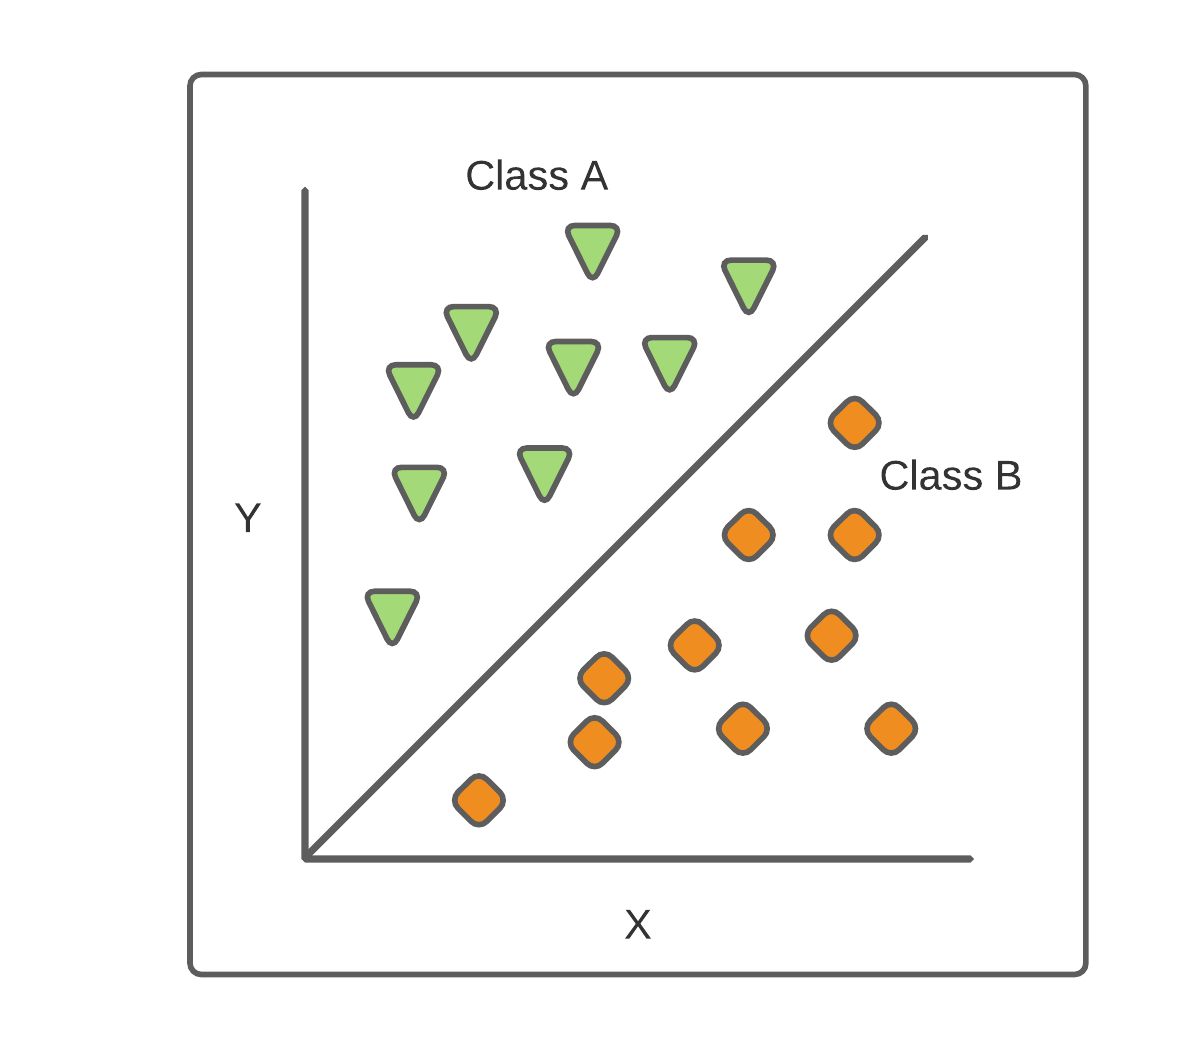
\includegraphics[scale=0.7]{classification-diagram.png}
					\caption{example of classification}
					\label{fig:classifcation}
				\end{figure}
			\subsection{Regression}
				Regression problems involve predicting a numerical value from the feature vector of an object.
				For example, given many variables about a stock (past history), predict the future value of the stock. Regression is
				about creating a mapping function from $\mathbb{R}^n \mapsto \mathbb{R}$. \par
				Let $x_n$ be a feature/parameter of the object and $k$ be the numerical value associated with it.\\
				Then a general regression function can be described as the mapping: \[[x_1,x_2,\cdots] \mapsto k\]
				\begin{figure}[h]
					\centering
					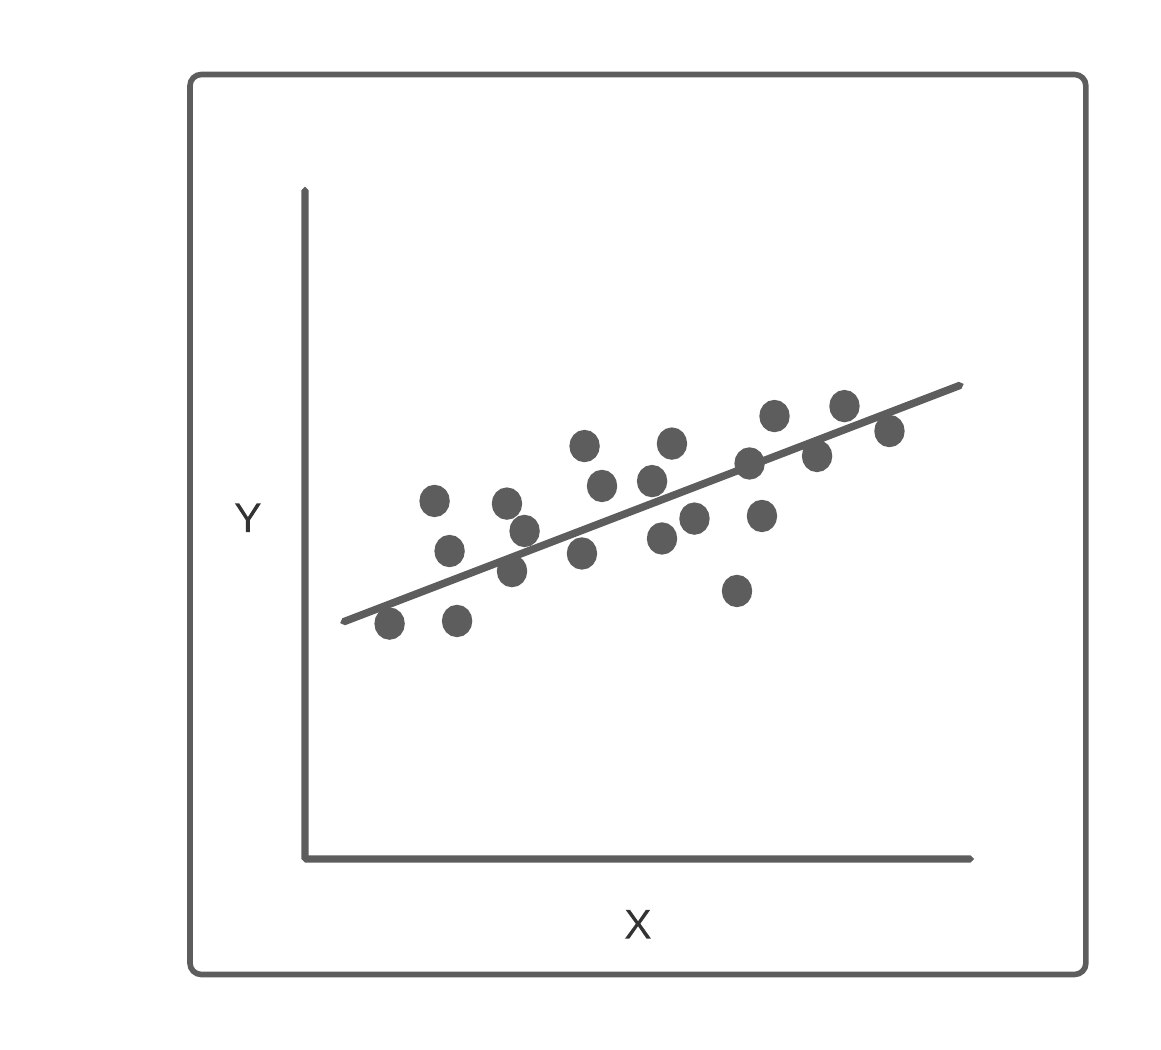
\includegraphics[scale=0.7]{regression-diagram.png}
					\caption{example of regression}
					\label{fig:regression}
				\end{figure}

		\section{General Optimization of Supervised Learning Problems}
			The optimization of supervised learning problems requires minimizing the average value of the loss function using the training samples. This produces the
			most accurate approximation to the underlying function to extrapolate values. \par
			The general equation \autocite[p. 3]{SurveyOfOptimizationMethods} for this can be written as:
			\begin{equation}
				\min_\theta \frac{1}{N} \sum_{i=1}^{N} L(y^i, f(x^i,\theta))
				\label{eq:supervised-learning-general}
			\end{equation}
			where $N$ is the number of training samples, $\theta$ is the parameter of the mapping function, $x^i$ is a feature vector
			and $y^i$ is the array of labels associated with that feature vector. \par
			The problem with using training samples is that the resulting function might be over-fitted to the given data. This would mean
			that, although the model is accurate for the training data it has been given, accuracy is reduced on new objects. A method to
			deal with this is through a regularization item, $\lambda$:
			\begin{equation}
				\min_\theta \frac{1}{N} \sum_{i=1}^{N} L(y^i, f(x^i,\theta)) + \lambda\| \theta\|_{2}^{2}
				\label{eq:supervised-learning-regularization}
			\end{equation}
			Regularization fundamentally discourages learning complex models \autocite[p. 4]{OverfittingSupervisedLearning}. The output will be affected by multiple features and as the number of features increases,
			the model becomes more complicated. Regularization will selectively favour the most significant features while minimizing the importance of features which have little effect on the final output.

		\section{Limitations of Supervised Learning}
			Models don't generalize well from observed, training data to unseen data \autocite[p. 1-3]{OverfittingSupervisedLearning}. The accuracy might be near perfect
			on training data while being poor on unseen data, somewhat mimicking the model memorizing the training data without grasping the mapping function. 	Many of the reasons for this can be attributed to the data set. \par
			Firstly is the problem of choosing a suitably sized dataset. Learning using only a small number of samples limits the accuracy since there is not enough data to realize
			any meaningful connections. A large amount of training with labelled data, while increasing the training accuracy, will decrease the overall
			accuracy of the model when validating unseen data (validation accuracy). This is because of diminishing returns - resulting from the learning speed slowing down - causing
			memorization instead of learning. Consequently, one of the considerations is to have the right size data set to alleviate the risk of under-fitting or over-fitting. An easy way
			to do this is to train the model in batches and, after each epoch, check the validation accuracy until the error rate starts to increase. \par
			The quality of the data heavily influences how effective the transition between training and validation will be. For example, using skew data (in the sense that
			the training samples don't represent the whole domain of input variables) will lead to a model that is accurate given niche combinations of variables and has to
			extrapolate on others. There is also some unpredictable instability in the data called noise. Reducing noise is key in ensuring an accurate model and requires
			the data set to be pruned so that there remains mostly high-quality accurate data. The problem with this is that a noise-free training set will be more inaccurate than a
			data set with some noise since the finished model will be processing unseen data that will have inherent noise. \par
			Finally, there has to be a realistic bound to the model's complexity. As more inputs are added, the model becomes more accurate on average but has lower consistency and
			will require more training data. The culmination of all these factors is that training data requires great resources to produce. Without considering where the unlabelled data is coming from,
			human intervention will be required to label the data which means that each label has to be calculated for potentially thousands or millions of training samples.
			Apart from the amount of time this takes, human error can be a great detriment to the quality of the data (measurement errors and mislabelling). Most of the time, producing a good
			model is limited by how much good data you can obtain.







	\chapter{Unsupervised Learning}

			\section{Application of Unsupervised Learning}
			Unsupervised learning is different to supervised learning in the way that it uses unlabelled data \autocite[p. 105]{DeepLearning}; instead
			of learning from a mapping of inputs to a known output, the model is given only the inputs to learn from and has to make sense of the data without guidance.
			As a result of this, unsupervised learning revolves around extracting relationships from the data without the inherent human biases caused by choosing the correct output beforehand. \par
			Unsupervised learning problems strive to solve 2 problems: finding clusters of similar data and summarizing the underlying distribution of the data
			(density estimation).

				\subsection{Clustering}
					Unlike classification, where the classes are predefined, clustering requires the model to define its own cluster of data
					based on the similarities of the features.
					\begin{figure}[h]
						\centering
						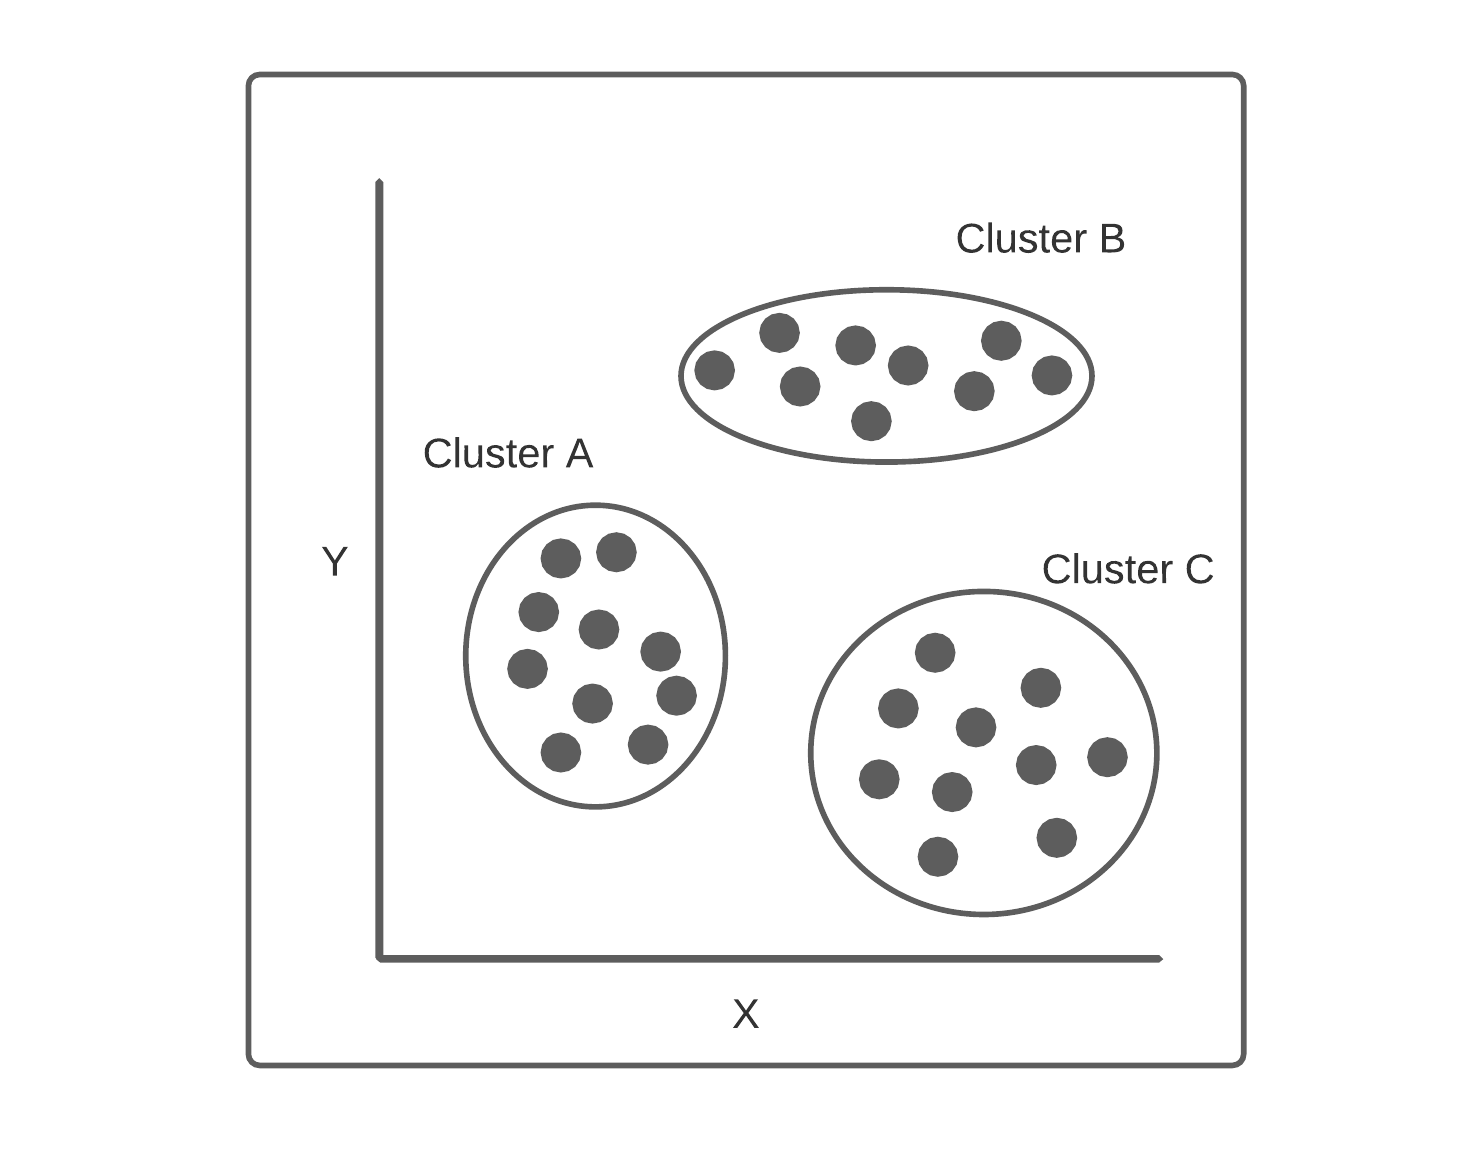
\includegraphics[scale=0.7]{clustering-diagram.png}
						\caption{example of clustering}
						\label{fig:clustering}
					\end{figure} \\
					Optimization will involve making the variance of each cluster as small as possible (variance will
					be equivalent to the distance from the centre of the cluster). This can be done by iterating through each cluster
					and checking the distance from the centre of the cluster for each sample.
					\begin{equation}
						\min_s \sum_{k=1}^{K} \sum_{x\in S_k} \| x - \mu_k \|_{2}^{2}
						\label{eq:unsupervised-learning-clustering}
					\end{equation}
					where $s$ is the variance, $K$ is the number of clusters, $S_k$ is the set of samples for that cluster,
					$\mu_k$ is the centre of a cluster \autocite[p. 3-4]{SurveyOfOptimizationMethods}.

				\subsection{Density Estimation}
					The assumption is that there exists some probability distribution to describe the relationship between the variables \autocite{sheather2004density}.
					Density estimation is a useful asset in modelling to estimate the properties of a given data set (variance, skewness, type of distribution). \par
					Suppose there exists a set of continuous random variables, $(x_1,\cdots,x_n)$, then there is a
					probability distribution that the set models, $P(x_1,\cdots,x_n)$. The goal is to find a probability density function (PDF)
					that can describe the mapping: $(x_1,\cdots,x_n) \to P(x_1,\cdots,x_n)$. The assumption that this will PDF will be continuous is valid
					since our objective function has the precondition of being continuous.
					\begin{figure}[h]
						\centering
						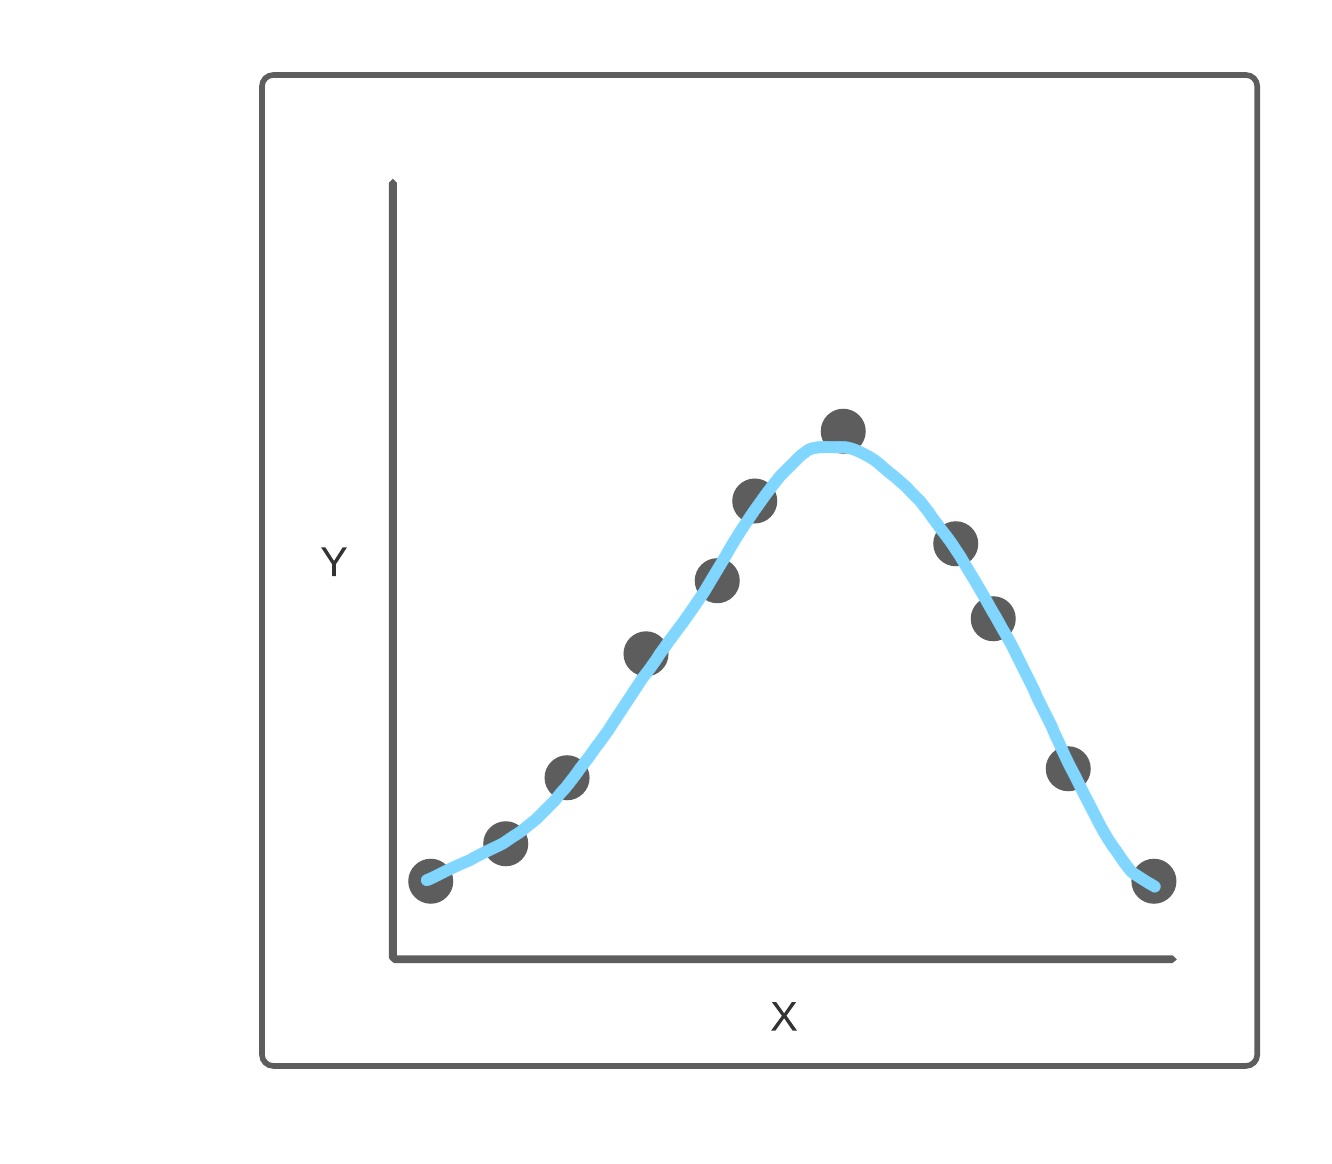
\includegraphics[scale=0.2]{density-estimation-diagram.jpg}
						\caption{example of density estimation}
						\label{fig:density-estimation}
					\end{figure} \\
					Getting the exact function for the data is not only unlikely but also suboptimal. As more data is used, the approximation will
					get more complex and usually closer to the actual value however too much data increases the risk of over-fitting to the data, especially if there is
					abnormal data. Instead, the focus is to maximize the likelihood that a predicted PDF is correct. \par
					In statistics, the likelihood function measure the goodness of fit between the data and the proposed PDF, so maximizing it finds the PDF which
					has the highest probability of fitting the data.
					A likelihood function is written as $p(x^i,\theta)$ where $x^i$ is a data point and $\theta$ is a PDF.
					However, many data sets have large  numeric ranges that can limit the effectiveness of this function so it is easier to work with the
					logarithmic likelihood function, $\ln p(x^i,\theta)$ or $\ell(x^i,\theta)$. \par
					It is important to note that
					\begin{equation}
						\max p(x^i,\theta) = \max \ell(x^i,\theta) = \widehat{\ell}(x^i, \widehat{\theta})
					\end{equation}
					Since $\ln$ is strictly increasing, maximizing the logarithmic likelihood function also maximizes the likelihood function. Thus general density estimation \autocite[p. 4]{SurveyOfOptimizationMethods} is:
					\begin{equation}
						\max \sum_{i=1}^N \ell(x^i,\theta)
					\end{equation}
					where $N$ is the number of training samples and $x^i$ is a particular feature vector of a sample.

			\section{Limitations of Unsupervised Learning}
				The quality of data is, just like in supervised learning, pivotal to the ability for the model to function. Although data
				doesn't need to be pre-processed and labelled in the same manner as supervised learning, unsupervised learning
				still has the shortfall of requiring data that is representative of the whole data set to prevent skew results. Furthermore,
				the data needs to have a suitable resolution for clustering. If the data has a small resolution then segments that represent separate clusters could be
				grouped. Consider data which represents clusters `$2-3$', `$4-5$' and `$95-100$' units. There is a possibility that the first 2 clusters are grouped as 1 cluster.
				Problems like these could be resolved by using a recursive method to analyse the clusters of each cluster but in the end the process will always be time-consuming. \par
				The nature of unsupervised learning - being the use of raw data - will lead to apprehension as to the usefulness and accuracy of the results. Without human intervention the
				practicality of the outputs will be greatly dependant on the model being used. Accuracy is generally lower than other learning options seeing that the model has to
				establish its own connections based on features in similarity with no notion as to whether they are correct. It is due to this fact that the relationships extracted have with no application. \par
				Finally, unsupervised tasks will require a far greater amount of data than their supervised counterparts. Extracting worthwhile relationships with no way to predefine the output
				of the model will require much more data to not only lessen the effect that outliers and abnormalities would have on the prediction but also to compensate for the complexity, which scales
				exponentially with each input variable added. \par
				It is as a consequence of these limitations that often unsupervised learning is less preferable to some hybrid models like semi-supervised learning which mixes labelled and unlabelled data
				to increase the chance of producing practical and relevant results.


	\chapter{Reinforcement Learning}
		Reinforcement learning entails an agent interacting with an environment rather than using a traditional dataset \autocite[p. 105]{DeepLearning}.
		The learning process is done through trial and error to develop a feedback loop between the environment and the agent's experience. Each state of the environment should be mapped to the action that maximizes the reward. \par
		This game theory approach assigns a payoff yield to each action that encourages or discourages certain actions.
		A by-product of this is to consider how the length of time can affect the payoff of an action. For example, maybe an action has
		a high reward when considering only the next state but when looking at the next 10 states its value is lower. This can be seen
		in chess when, as the depth of the AI get higher, certain moves become worse as they compromise future positions. \par
		The dynamic nature of reinforcement learning is useful in complex systems where computationally working out the whole game would be inefficient if not impossible.
		Consider chess \autocite{shannon1950xxii} where the number of possible games is estimated as $10^{123}$ (Shannon's number) and is too big to compute effectively after even 5 turns.
		\begin{figure}[h]
			\centering
			\begin{tabular}{||c c||}
				\hline
				Number of half-moves & Number of Possible Games\\ [0.5ex]
				\hline\hline
				1 & 20\\
				\hline
				2 & 400\\
				\hline
				3 & 8,902\\
				\hline
				4 & 197,281\\
				\hline
				5 & 4,865,609\\[1ex]
				\hline
			\end{tabular}
			\caption{the exponential growth of possible chess games}
			\label{fig:possible-chess-games}
		\end{figure}


		\section{Optimization in Reinforcement Learning}
			A policy function, $\pi(s)$, maps a state, $s$, to an action, $a$, to select the best course of action from the set of all actions, $A$, that the agent
			can take in each situation from the set of possible situations, $S$.
			\[\pi(s) : s \to a \ \text{where} \ s\in S, a \in A\]
			By maximizing the expected value of this function \autocite[p. 4]{SurveyOfOptimizationMethods}, the agent will select the
			best action to be performed in each state, maximizing the payoff of the actions.
			\begin{equation}
				\max_{\pi(s)} = \mathbf{E} \left[\sum_{k=1}^{T} \gamma^k r_{t+k} | S_t = s \right]
				\label{eq:reinforcement-learning}
			\end{equation}
			where $T$ is the time horizon, $\gamma$ is the discount factor, $r$ is the reward function with respect to the turn and
			the time into the future being considered, $S_t$ is a given state. \par
			If the game was infinite - or has no predetermined stopping point -
			then a simple solution is to work out the $\lim_{T \to \infty}$ and truncate the series at some point to get a good approximation.
			Using this method of truncation would allow the depth to be changed (how far into the future turns are considered). \par
			The discount factor, $\gamma$, is a value that prioritizes instant reward over a future reward \autocite{sozou1998hyperbolic}.
			If there is a constant risk which may cause failure to realize the reward then that future reward should
			have a decreased payoff to compensate for the risk. For example, suppose there is a 50\% chance (implying $\gamma = 0.5$) that the game ends after every
			turn and you could choose either a payoff of 1 unit after 1 turn or a payoff of 10 units after 5 turns. Then the expected value of option 1 is
			$0.5^1 \cdot  1$ which is 0.5 and option 2 is $0.5^5 \cdot  10$ which is 0.3125 so option 1 is statistically better.

		\section{Limitations of Reinforcement Learning}
			A noisy environment will cause a sharp decrease in learning speed. If feedback is delayed (like the effect of an action doesn't happen until a few time intervals after)
			then differentiating cause and effect can be difficult. Unlike data sets, where the noise can be artificially removed, there is no possibility of removing
			this noise since then the environment would be different and the agent would be acting on an unrelated environment. It is because of this that the efficacy
			of the model will fluctuate as new game theory is being developed. Whenever new strategies are tried, the performance might decrease in the short term however
			the trial-and-error process will encourage a greater depth of strategy later. \par
			Many of the parameters of an environment will have to be manually set. For example, the correct value for the discount factor is
			usually obvious - as close to 1 as possible for continuos environments and otherwise the risk every time step - but realistically there has
			to be some focus on short term rewards as an extremely long wait is not conducive to real life. This can be seen in chess where three-fold repetition
			and the 50 move rule (no captures or pawn moves in 50 turns) will result in a draw. In this case, there is a preset condition that prevents the best moves
			being played if the time scale is too large. \par
			The subjective nature of payoffs is also pertinent to the development of a simulation. As systems get more complex it becomes more difficult to ascribe
			values to the actions that can be taken. Either these values will follow some subjective set of rules, in which case they are still influenced by some bias, or they
			must be chosen subjectively thus human bias creates preferred ways to operate leading to a sub-optimal set of actions. \par
			 One way to minimize human bias and thus
			reach the optimum solutions is to simplify the outcomes. For instance, in chess, the set of outcomes and payoffs can be reduced to a positive payoff for a win and a
			negative payoff for a loss without considering the possible decisions to get there. This methodology, when paired with deep learning, will lead to the computer playing
			many games with itself to work out the relative payoffs and tweak them over time as new strategies eclipse old ones. Over millions of games and multiple generations
			of neural networks, the result will be a model with the optimum policy function that has as little human bias as possible and therefore can express actions that would
			naturally be unorthodox or creative. The downside of this is the resources and time required to reach this transcendental state in a reasonable time frame.


	\chapter{Mathematical Models for Optimization}

		\section{Constraints on the Objective Function}
			Constraints are conditions that the solutions to the objective function must satisfy. In many cases, there are
			certain restrictions that should be added due to computational and resource limitations. \par
			There are 3 types of constraints that must be considered:
			\begin{itemize}
				\item inequality constraints such as $x \geq k$.
				\item equality constraints such as $x = k$
				\item data type constraints such as $x$ is an integer ($x \in \mathbb{Z}$)
			\end{itemize}
			Data type constraints are normally easy to deal with; changing with values the model checks or adding a conditional statement
			can be enough in many cases. \par
			Equality constraints can be appended onto the objective function using the Lagrange multiplier \autocite{LagrangeMultiplier}. Let
			$f(x)$ be an objective function and $c_{n}(x) = k_n$ be an equality constraint. Then the general Lagrange multiplier for $n$ constraints would be:
			\begin{equation}
				\mathcal{L} (x) = f(x) - \lambda_1(c_{1}(x) - k_1) - \cdots - \lambda_n(c_{n}(x) - k_n)
			\end{equation}
			The solution to the original objective function, $f(x)$ will be a saddle point on the Lagrange multiplier. One problem with this
			approach is that, firstly, for each constraint added there will be an extra partial derivative that needs to be computed and thus a more
			complex simultaneous equation. In addition, inequality constraints ($c(x) \geq k$) are not supported through this method. However, there
			is a generalization to the Lagrange multiplier called the Karush–Kuhn–Tucker (KKT) conditions.

		\section{Methods for Finding Extrema}
			\subsection{Jacobian}
				Previously, it was ascertained that the locations of the critical points required the first derivative of the function to be 0 ($f' = 0$).
				For a single-valued function this is equivalent to solving \[\frac{dy}{dx} = 0\]
				However for multi-valued functions a critical point will require all partial derivatives to be 0 at that point. The Jacobian \autocite{Jacobian} is
				a vector of the partial derivatives of the function that gives a vector of the gradients at that point.
				\begin{equation}
					J_f = \nabla f = [\partial_{x_1} f, \cdots, \partial_{x_n} f]
					\label{eq:jacobian}
				\end{equation}
				This can be solved by either setting each partial derivative to 0 and solving it simultaneously or by finding the values
				when the value of the Jacobian is 0. \[\partial_{x_1} f = \cdots = \partial_{x_n} f = 0 \ \textrm{or} \ \| J \| = 0 \]
				Sometimes the resulting equations might be difficult to solve (polynomials of order greater than 4 for example) and brute force or numerical methods
				might need to be used.
			\subsection{Hessian}
				After finding the locations of the critical points, higher-order derivative tests must be used to determine the nature of the points.
				The Hessian \autocite{Hessian} is like the 'Jacobian of the Jacobian' and is a representation of the change in the gradient.
				\begin{equation}
					H_f = \nabla(\nabla f) =
						\begin{bmatrix}
							\frac{\partial^2 f}{\partial x_{1}^{2}} & \frac{\partial^2 f}{\partial x_1 \partial x_2} &\cdots & \frac{\partial^2 f}{\partial x_1 \partial x_n}\\
							\frac{\partial^2 f}{\partial x_2 \partial x_1} & \frac{\partial^2 f}{\partial x_{2}^{2}} & \cdots & \frac{\partial^2 f}{\partial x_2 \partial x_n}\\
							\vdots & \vdots  & \ddots & \vdots \\
							\frac{\partial^2 f}{\partial x_n \partial x_1} & \frac{\partial^2 f}{\partial x_n \partial x_2} & \cdots & \frac{\partial^2 f}{\partial x_{n}^{2}}
						\end{bmatrix}
					\label{eq:hessian}
				\end{equation}
				Due to the commutative nature of second partial derivatives, computation time is significantly cut down as only the upper or lower
				triangular matrix has to be calculated and then mirrored.
				\begin{equation}
					\frac{\partial^2 f}{\partial y \partial x} = \frac{\partial^2 f}{\partial x \partial y}
					\label{eq:symmetry}
				\end{equation}
			\subsection{Higher-Order Derivative Tests}
				Using the determinant and trace of the Hessian matrix where $\lambda$ is an eigenvalue
				\begin{equation}
					trH = \sum_{i=1}^n H_{ii} = \sum_{\forall i} \lambda_i \ \text{and} \ detH = \prod_{\forall i} \lambda_i
				\end{equation}
				the second derivative test is as follows.
				Let $(x_1,x_2,\cdots,x_n)$ be a critical point substituted into the Hessian. Then \autocite{SecondDerivativeTest}
				\begin{itemize}
					\item $detH > 0$ and $trH > 0 \implies$ local minimum.
					\item $detH > 0$ and $trH < 0 \implies$ local maximum.
					\item  $detH < 0 \implies$ saddle point.
					\item $detH = 0 \implies$ inconclusive test.
				\end{itemize}
				Doing this for all critical points will determine which are extrema and comparing the values of the extrema will find the global
				minimum or maximum, which will be the solution to the optimization problem. In the case when the test is inconclusive, higher-order
				tests \autocite{ExtremumTest} can be used (although many derivatives would have to be calculated) or inspection. \par
				For complex functions, visual inspection is usually impossible (since displaying something with greater than 3 dimensions is unintuitive) but numerical inspection can be useful, like
				adding $dx_n$ for each variable and comparing the values. For example, if the neighbourhood of a point has values greater than the point it must be a minima. \par
				The Hessian matrix is not without limitations; the computing time required to work out the Hessian scales greatly as each new variable is added and, for each critical
				point, the eigenvalues of the matrix will have to be worked out to find the trace and determinant. To mitigate this there are algorithms that can approximate the Hessian
				with the only condition that the matrix is invertible (the determinant is not 0).

			\subsection{Iterative Methods}
					When exact solutions are too difficult to calculate either due to too many variables or the Hessian matrix being to large
					to reasonably store, iterative methods can be used as numerical approximations. Since the approximation will converge to the
					answer as the number of iterations approaches infinity, many iterative methods are far superior, in practice, because of the lower
					resource cost relative to the accuracy of the approximation. \par
					Newton's method for finding extrema \autocite{fletcher2013practical} is one of the most simple of the iterative methods
					and demonstrates many downfalls of early iterative formulae.
					\begin{equation}
						x_{k+1} = x_k - \frac{f'(x_k)}{f''(x_k)}
						\label{eq:newtons-method-single}
					\end{equation}
					or in the case of multi-valued functions
					\begin{equation}
						x_{k+1} = x_k - [H_f(x_k)]^{-1} J_f(x_k)
						\label{eq:newtons-method-multi}
					\end{equation}
					where $H^{-1}$ is the inverse Hessian and $J$ is the Jacobian. Considering the preconditions, this technique is still quite limited.
					Although we don't have to solve simultaneous equations or compute a derivative test, the Hessian has to be calculated and inverted (which requires it to be non-singular). \par
					More importantly, this sequence will only converge to one value even if the function has multiple critical points. The initial guess, $x_0$,
					has a huge impact on where the sequence converges assuming it converges. In this sense, Newton's method has the
					property of local convergence where the sequence will converge when $x_0$ is close to a critical value. \par
					A few other things to consider are that the convergence point might be a saddle point rather than an extrema and sometimes the sequence might
					not converge but rather cycle between values without settling on the extrema. Most of the problems stem from choosing a bad starting point or
					discontinuous derivatives. \par
					Many of these issues are addressed in more modern algorithms (each with their limitations).
					To reduce the computational resources required, quasi-newton methods use update formulas to approximate the Hessian at every step, reducing the time and space complexity of each iteration.
					Many different update formulas are used situationally. On the other hand, to reduce the effect of bad starting points, stochastic methods (like stochastic gradient descent)
					choose starting points randomly while reducing convergence time to compensate. \par
					The reality is that there are many ideologies behind iterative optimization that
					all preserve the same concept of finding a series converging on a solution.

\listoffigures
\printbibliography[title=References]
\end{document}
